%! Author = sbbfti
%! Date = 10/06/2020

% \subsection{Models}
% \textit{finish} \kla{reviewers could argue that some other models learn both syntactic and semantic information. If this model only learns syntactic, how are they going to be accurate? check existing work why they call they learn semantic information and see if ours also learn semantic information or not. Otherwise, we are downtown the claim.}

% \kla{should we talk about two prediction tasks somewhere? Task1=? and Task2=}

\subsection{(Step 4) Multi-Task Training Architectures}
\label{sec:approach-arch}


% On the other hand, training multiple single models on multiple tasks is also possible, but predictions are competing and the multiple sources of information are not jointly learned together, leading to inaccurate predictions.



Our \our~leverages a Multi-Task Training (MTT) paradigm, which is a set of techniques designed to learn multiple tasks, allowing the model to capture multiple sources of information.
Traditionally, deep learning is designed for one single learning objective (e.g., only predicting the next code token), limiting its ability to capture other important and useful sources of information (e.g., syntactic information of source code).
Instead of training a model with one single learning objective, the MTT paradigm aims to provide a generalist model with multiple learning objectives, providing a more robust vector representation.
For our \our~approach, we design the target task to predict the next token, while the supporting task (aka. an auxiliary task or additional related non-target task) is to predict the token type.
In addition, we build three variants of \our, with three different MTT techniques, according to two learning styles~\cite{phang2018sentence} as follows.
% (i.e., \our-Hard, \our-Soft, and \our-IFN)

\subsubsection{Multi-Task Learning (MTL)}

Multi-Task Learning (MTL) is an MTT technique to learn multiple tasks simultaneously instead of learning them separately.
Normally, during the learning process, the model aims to optimize a loss function for one single learning objective.
With the MTL approaches, multiple loss functions are optimized together during the learning process, allowing the MTL-based model to simultaneously learn against multiple objectives and share the knowledge understanding from multiple related sources.
In this paper, we consider two main MTL approaches for Multi-Task Learning (MTL)~\cite{ruder2017overview}, i.e., Hard Parameter Sharing (\our-Hard) and Soft Parameter Sharing (\our-Soft).

For \emph{Hard Parameter Sharing}, the key principle is to train a code completion model against two learning objectives, where the loss functions of the two learning objectives ($L_{code}$ and $L_{type}$) are optimized together within the same model.
Formally, the \our-Hard model aims to minimize the following loss function: 
\begin{equation}
    \label{eq:1} 
    \begin{aligned}
    \medmath{L_{Hard} = \argmin_{\omega}(L_{code}(d_{code}, \omega) + L_{type}(d_{type}, \omega))}
    % loss_{hardShare} = codeLoss + typeLoss
    \end{aligned}
\end{equation} 

\noindent , where $d_{code}, d_{type}$ denotes the code token dataset and the token type dataset, respectively, and $\omega$ denotes a model's parameters.
With Hard Parameter Sharing, the weights and model parameters are shared between tasks, allowing the model to explicitly learn the input representations between tasks (i.e., code and type vectors) that are closely related.



% via the shared layers which may help enhance the effectiveness of the target task's results.
% After the shared layers, usually there are separated task-specific output layers for each task.
% However for our work, the tasks have similar outputs i.e. tokens from the vocabulary.
% Therefore, we train both target task and supporting task in the same model simultaneously without separated output layer.

% SynComp hard parameter sharing uses one GPT-2 model with two losses: code prediction loss ($L_{code}$) and type prediction loss ($L_{type}$).
% The model minimize the summation of losses shown in Equation~\ref{eq:1}.



% For hard parameter sharing, the tasks will share the same model backbone which mean the weights and parameter of the model being shared together.
% Only the task-specific output layer that might be different.
% A hard parameter sharing model is one of the most popular multi-task learning techniques.
 

% \kla{wannita will write soft....}

% \subsubsection{MTL: Soft Parameter Sharing Model}
% For soft parameter sharing, each task will have its own model backbone, i.e. separate weights and parameters.
% However, the models are loosely connected by the constraint which try to minimize the distance of the model parameters' difference.
% This is to regularize the model parameters to be similar.
For \emph{Soft Parameter Sharing}, the key principle is similar to Hard Parameter Sharing where the goal is to train a code completion model with two learning objectives.
However, instead of training a model against two tasks like the Hard Parameter Sharing model, the Soft Parameter Sharing is designed to train two individual models for each task ($L_{code}$ and $L_{type}$), allowing each model to learn separately for each task.
Therefore, each learning objective has an individual model (i.e. separated weights and parameters between the learning objectives).
% to learn and predict outputs; 
To allow the model to share the knowledge between tasks (i.e., to learn the similarities between the related parameters), a shared loss function is also used, which is computed as follows:

\begin{equation}
    \label{eq:norm}
    L_{sharing}(\omega_1, \omega_2) = 
    % ||W||_F = 
    \sqrt{\sum_{i=1}^{I}\sum_{j=1}^{J}|\omega_{1(i,j)}-\omega_{2(i,j)}|^2}
\end{equation}

% Nonetheless, the models are loosely connected by the constraint to encourage similarities between related parameters.


% The constraint ($L_{sharing}$) which is used to optimize the difference of distance between the models parameters' applies with Frobenius norm:

\noindent , where $\omega_n$ denotes the model parameters of the  learning objective $n$. Finally, the \our-Soft model aims to minimize the following loss function:

\begin{equation}
\label{eq:2}
\begin{aligned}
    L_{Soft} = \argmin_{\omega_1, \omega_2}
    &( L_{sharing}(\omega_1, \omega_2)\\ 
    &+ L_{code}(d_{code}, \omega_2)\\
    &+ L_{type}(d_{type}, \omega_1))
\end{aligned}
\end{equation}

With Soft Parameter Sharing, each learning objective has its own model parameters and weights, allowing the models to implicitly learn the input representations that might have more connection to a specific task.

% SynComp soft parameter sharing uses two GPT-2 models with three losses: code prediction loss, type prediction loss, and sharing loss. The model minimize the summation of losses shown in Equation~\ref{eq:2}.

\subsubsection{Intermediate Fine-Tuning (IFT)}

\emph{Intermediate Fine-Tuning (IFT)}~\cite{phang2018sentence} adapts a transfer learning concept (i.e., pre-training then fine-tuning) where the goal is to learn multiple tasks sequentially. First, the model is fine-tuned on the supporting task (token type prediction) followed by the target task (code token prediction), respectively.
Thus, the fine-tuned step on the supporting task can be considered the second stage of the model pre-training.
Therefore, the Intermediate Fine-Tuning (IFT) model (\our-IFT) is first trained based on an intermediate self-supervised task (token type prediction), then trained on the target task (code token prediction), allowing the model to gain knowledge on the token type prior to predicting the next code tokens.


\subsection*{GPT-2 Model Architecture}

Among the three variants of the MTT techniques (i.e., \our-Hard, \our-Soft, and \our-IFT), we use the GPT-2 architecture as a base model.
GPT-2~\cite{radford2019language} is a decoder-only Transformer model.
The GPT-2 architecture for code completion consists of three main components: the embedding layer, the decoder block, and the language model head. 
First, the embedding layer embeds the input tokens into vectors with positional encoding, allowing the model to learn the semantic meaning and the position of each code token.
Then, the embedding vectors are fed into the decoder block which contains decoder layers.
Each decoder layer includes masked self-attention layers, feed-forward neural network layers, and normalization layers.
%  It basically always scores the future tokens as 0 so the model can’t peak to future words
The masked self-attention layer indicates which tokens to focus on, while the masking approach prevents the attention mechanism~\cite{vaswani2017attention} to see the unseen tokens in the future.
% \kla{wannita will do the rest}.
% Feedforward neural nets are complex network made up an input layer that accepts information, hidden layers that capture the hidden correlations between each data point, and an output layer which transmit information.
The feed-forward neural network layer is a sophisticated network with hidden nodes to capture the related information between each data point.
% Layer normalization (LayerNorm) is a technique to normalize the distributions of intermediate layers. It enables smoother gradients, faster training, and better generalization accuracy.
The normalization layer makes the learning process more effective by enabling smoother gradients and generalized accuracy.
% The linear layer takes the output of the last decoder block and converts it to a vector whose dimensions are vocabulary size by 1. In short, it takes a lot of inputs and produces a list where each spot represents a token. The higher the number in the spot the better the chance that that token is the best pick. Softmax converts the output of the linear layer to a probability distribution
After $L$ layers of decoder, an output of the last layer is fed to the language model head, i.e. a linear layer, which converts the output to a vector whose dimensions are the same as the vocabulary size.
Lastly, the vector is converted to a probability distribution by the softmax activation function.
Formally, to predict the next token $x_t$ based on a given input sequence, GPT-2 can be represented as follows:

\begin{equation}
\begin{aligned}
    \label{eq:transformer}
    h_0 &= W_e \cdot C + W_p \\
    % \label{eq:transformer2}
    h_l &= decoder\_layer(h_{l-1}), \forall l \in [1,L] \\
    % \label{eq:transformer3}
    P(x_t) &= y_t = softmax(h_n \cdot W^T_e), t \in [0, N]
\end{aligned}
\end{equation}

\noindent, where $W_e$ is the tokens embedding matrix, $C$ denotes the context vector of tokens, $W_p$ is the position embedding matrix, $L$ is a number of decoder layers, and $N$ is the length of the sequence.
We follow the traditional language models by maximizing the log-likelihood of:

\begin{equation}
    \label{eq:log-likelihood}
    L(x_t) = \sum_i{\log P(x_i|x_1...x_{i-1}, \omega)}
\end{equation}

\noindent, where $\omega$ is the model parameters that are learned during the optimization process.
Particularly, \our~uses the pre-train CodeGPT~\cite{lu2021codexglue} that is pre-trained on the CodeSearchNet dataset~\cite{husain2019codesearchnet} as a starting checkpoint.


% Below we provide details for each training techniques.



% In Fig.~\ref{fig:overview} shows the architectures of all described models.
% During the training phase, both tasks are cooperatively trained; however, the task can separately predict in the inference phase as shown in Fig.~\ref{fig:overview}.
% In other words, the token type information is used only to support throughout the training phase requiring no token type extraction in the inference phase.
% which yield to the benefit of on-the-fly model by not requiring token type extraction in the inference phase.

% SynComp has GPT-2~\cite{radford2019language}, a Transformer decoder-only model, as a based model for all techniques.
% The based model consist of three main components: embedding layer, decoder block, and language model head. 
% Before handing that to the first block in the model, we need to incorporate positional encoding – a signal that indicates the order of the words in the sequence to the transformer blocks.



% \gls{ifn} is adapted from transfer learning paradigm which is about pre-training and then fine-tuning on target task.
% Specifically, this is the training technique for sequential training.
% The model is fine-tuned on supporting tasks and then target task respectively.
% This technique benefit the model to learn the second stage of pre-training with intermediate supervised task that might mitigate the brittleness and improve the robustness and performance of the target task~\cite{phang2018sentence}.

% In our case, SynComp intermediate fine-tuning uses one GPT-2 model with the token type prediction as the supporting task. 
% Thus, we first fine-tune our \gls{ifn} model on type dataset.
% Then we fine-tune the same model again on code prediction task.




% Recently, both MTL approaches are used in code completion.
% For example, Liu~\ea~\cite{liu2020self, liu2022unified, liu2020multi} leverage Hard Parameter Sharing, while CodeFill~\cite{izadi2022codefill} leverage Soft Parameter Sharing.




% Typically, there are two approaches for training \gls{mtl}: hard parameter sharing and soft parameter sharing~\cite{ruder2017overview}.

% Basically, the inspiration to train the tasks at the same time on one or many models with jointly conditions.
% On the other hand, \gls{ifn} is the model training technique for \emph{sequential} training.

% Specifically, the model is fine-tuned sequentially on each supporting tasks, and then the target task respectively~\cite{phang2018sentence}.

% \subsubsection{Intermediate Fine-Tuning}

% To achieve this, we consider the following three MTT training techniques~\cite{phang2018sentence}.




% Some code completion research starts to apply \gls{mtl} with different tasks and datasets~\cite{izadi2022codefill, liu2020self, liu2022unified, liu2020multi}.
% Particularly, most of the time \gls{mtl} has been used for \gls{ast} training~\cite{izadi2022codefill, liu2020self, liu2022unified} in order to learn syntactic information of source code.
% However, the source code of code completion task is usually incomplete or syntactically incorrect which leads to the limitations of extracting \gls{ast} data in practice (section 2.2).
% To address the limitations of previous works, our work
% % is the first to
% leverages \gls{mtl} with \emph{token type} information that represent the light-weight syntactic information and is more flexible to be extracted. 
% Moreover, although showing benefits in many NLP research~\cite{phang2018sentence, weller2022use, gururangan2020don}, to the best of our knowledge \gls{ifn} has never been introduced to code completion field.
% Therefore, this motivate us to include the technique to our experiment along with \gls{mtl}.







% PyCoder-Hard
% PyCoder-IFT

% However, sometimes the additional related non-target tasks (i.e. supporting task or auxiliary task) are presented with the intention of improving the target task's performance.
% When supporting task has been presented during the fine-tuning stage, there are multiple techniques to combine or alternate between these target task and supporting task -- such techniques can be called \emph{multi-task training techniques}.


% at the same time rather than separately.

% target dataset
% supporting dataset



% In the past, pre-train language model and fine-tune on target task has become the standard paradigm for NLP~\cite{raffel2020exploring} and also be adapted to many tasks in software engineering~\cite{wang2021codet5, feng2020codebert}.

% These kind of tasks are called supporting task or auxiliary task.
% However, when non-target tasks has been presented more than one


% Recently in NLP, there is a study for how to best make use of the supporting data~\cite{weller2022use}.
% Two predominant methods used are \gls{mtl} and \gls{ifn}. 
% \gls{mtl} is a model training technique for \emph{simultaneous} training.
% Typically, there are two approaches for training \gls{mtl}: hard parameter sharing and soft parameter sharing~\cite{ruder2017overview}.
% Basically, the inspiration to train the tasks at the same time on one or many models with jointly conditions.
% On the other hand, \gls{ifn} is the model training technique for \emph{sequential} training.
% Specifically, the model is fine-tuned sequentially on each supporting tasks, and then the target task respectively~\cite{phang2018sentence}.



% \subsubsection{MTL: Hard Parameter Sharing Model}
% For hard parameter sharing, the tasks will share the same model backbone which mean the weights and parameters of the model being shared together.
% Only the task-specific output layer that might be different.
% A hard parameter sharing model is one of the most popular multi-task learning techniques.
% This technique completely shares the model backbone (i.e. weights and parameters) between tasks.
% The benefit is that the model could \emph{explicitly} learn the input representations between tasks via the shared layers which may help enhance the effectiveness of the target task's results.
% After the shared layers, usually there are separated task-specific output layers for each task.
% However for our work, the tasks have similar outputs i.e. tokens from the vocabulary.
% Therefore, we train both target task and supporting task in the same model simultaneously without separated output layer. 

% SynComp hard parameter sharing uses one GPT-2 model with two losses: code prediction loss ($L_{code}$) and type prediction loss ($L_{type}$).
% The model minimize the summation of losses shown in Equation~\ref{eq:1}. where $d_{code}, d_{type}$ denotes code and type dataset respectively, and $\omega$ denotes a model's parameter.


% \begin{equation}
%     \label{eq:1} 
%     \begin{aligned}
%     \medmath{L_{hardShare} = \argmin_{\omega}(L_{code}(d_{code}, \omega) + L_{type}(d_{type}, \omega))}
%     % loss_{hardShare} = codeLoss + typeLoss
%     \end{aligned}
% \end{equation} 

% \subsubsection{MTL: Soft Parameter Sharing Model}
% For soft parameter sharing, each task will have its own model backbone, i.e. separate weights and parameters.
% However, the models are loosely connected by the constraint which try to minimize the distance of the model parameters' difference.
% This is to regularize the model parameters to be similar.
% A soft parameter sharing model has particular model backbones for each objective task, i.e. separated weights and parameters.
% Each model learns and predicts results nearly independently; to be precise, there are loosely connected by the constraint to encourage similarities between related parameters.
% More specifically, the model is trained on each task individually along with penalizing on the distance between the model parameters' difference.
% The benefit of this technique is that each task has its own model parameters, so the model \emph{implicitly} learn the input representations and might have more connection to a specific-task.
% This constraint is expressed as \emph{sharingLoss} ($L_{sharing}$). 
% In this work, we apply the square Frobenius norm in Equation~\ref{eq:norm} as the \emph{sharingLoss}.

% \begin{equation}
%     \label{eq:norm}
%     ||W||^2_F = \sum_{i=1}^{I}\sum_{j=1}^{J}|w_{i,j}|^2
% \end{equation}

% SynComp soft parameter sharing uses two GPT-2 models with three losses: code prediction loss, type prediction loss, and sharing loss. The model minimize the summation of losses shown in Equation~\ref{eq:2}.
% \begin{equation}
% \label{eq:2}
% \begin{aligned}
%     L_{softShare} = \argmin_{\omega_1, \omega_2}
%     &( L_{sharing}(\omega_1, \omega_2)\\ 
%     &+ L_{code}(d_{code}, \omega_2)\\
%     &+ L_{type}(d_{type}, \omega_1))
% \end{aligned}
% \end{equation}

% \begin{equation}
%     \label{eq:2}
%     loss = \alpha * codeLoss + \beta * typeLoss + (1 - \alpha - \beta) * sharingLoss
% \end{equation}

% \subsubsection{STILTs: Intermediate Fine-tuning}
% From pre-training on supporting task, and then fine-tuning on the target task;
% this training technique apply the same paradigm method but with many supporting tasks called auxiliary tasks.



% \kla{move from background / will revise later}
% \emph{SynComp} leverages a multi-task training model, focusing on two training tasks: source code prediction (semantics information), and token type prediction (syntactic information).
% While the code prediction is a target task, the type prediction is a supporting task.
% SynComp explores on 3 multi-task training techniques: (3.4.1)~MTL: Hard Parameter Sharing Model, (3.4.2)~MTL: Soft Parameter Sharing Model, and (3.4.3)~\gls{ifn}: Intermediate Fine-tuning Model.
% Supplementary Training on Intermediate Labeled-data Tasks Model.



% Therefore, the training phase consist of 2 tasks: source code prediction and token type prediction.
% There are multiple techniques to learn such target task (source code prediction) with auxiliary task (type prediction). However, SynComp is inspired by weller~\ea~\cite{weller2022use} to leverage the usage of \gls{mtl} and \gls{ifn} training techniques. 

% \kla{why these three types are chosen? why do we need to explore these? - could cited~\cite{weller2022use} in the previous paragraph be the reason?}

% There are two dominant approaches in \gls{mtl} which are \emph{(3.3.1) hard parameter sharing model} and \emph{(3.3.2) soft parameter sharing model}. The core idea of both techniques is to learn the hidden robust representations from related tasks.

% \textbf{\gls{gtt}}
% We have 2 objective tasks here. First, the main task is code prediction and second task is type prediction as the auxiliary task. Both tasks, the models learn to predict in single-token level. Therefore when using in token-level prediction, the model can be used directly. For line-level prediction, the models are the same as in token-level prediction, however, are set to prediction until stop criteria is reached.


% \textit{finish} \kla{it would be great if we can discuss the advantages/disadvantages of each model? why we use them? why others are not explored? how are they different? }

% \textit{finish} \kla{I think we haven't talked about CodeGPT yet. Why using CodeGPT, instead of GPT-2? What is the limitation of CodeGPT? }
% We decide to include this method because the evidence shows that \gls{ifn} and \gls{mtl} are competitive and useful in some different scenario. If auxiliary task is larger than the target task, \gls{ifn} tend to perform better than \gls{mtl} \cite{weller2022use}. However, our type dataset is smaller than code dataset due to the tokenization process which all types are added in as the special tokens (see session 4.2). But we still choose to train \gls{ifn} in order to test the argument on the code completion task. We don't use repeated type dataset (see session 4.1) because dissimilar to \gls{mtl}, \gls{ifn} doesn't train code and type prediction simultaneously so we would like to maintain the granularity of data as normal.

% \begin{figure}[]
%     \centering
%     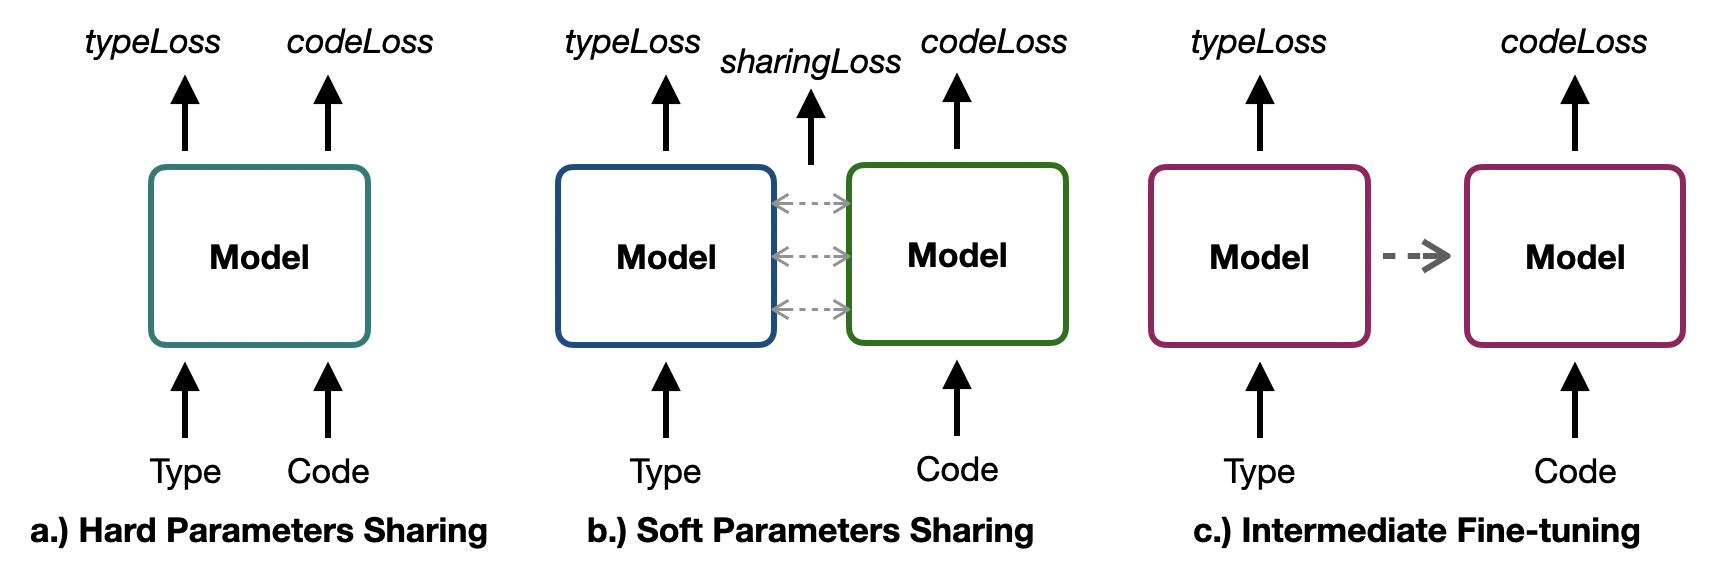
\includegraphics[width=\columnwidth]{figures/model_arch.png}
%     \caption{Model architectures (tentative pic)}
%     \label{fig:arch}
% \end{figure}